\documentclass[journal,12pt,twocolumn]{IEEEtran}

\usepackage{setspace}
\usepackage{gensymb}
\singlespacing
\usepackage[cmex10]{amsmath}

\usepackage{amsthm}

\usepackage{mathrsfs}
\usepackage{txfonts}
\usepackage{stfloats}
\usepackage{bm}
\usepackage{cite}
\usepackage{cases}
\usepackage{subfig}

\usepackage{longtable}
\usepackage{multirow}

\usepackage{enumitem}
\usepackage{mathtools}
\usepackage{steinmetz}
\usepackage{tikz}
\usepackage{circuitikz}
\usepackage{verbatim}
\usepackage{tfrupee}
\usepackage[breaklinks=true]{hyperref}
\usepackage{graphicx}
\graphicspath{ {./figures/} }
\usepackage{tkz-euclide}

\usetikzlibrary{calc,math}
\usepackage{listings}
    \usepackage{color}                                            %%
    \usepackage{array}                                            %%
    \usepackage{longtable}                                        %%
    \usepackage{calc}                                             %%
    \usepackage{multirow}                                         %%
    \usepackage{hhline}                                           %%
    \usepackage{ifthen}                                           %%
    \usepackage{lscape}     
\usepackage{multicol}
\usepackage{chngcntr}

\DeclareMathOperator*{\Res}{Res}

\renewcommand\thesection{\arabic{section}}
\renewcommand\thesubsection{\thesection.\arabic{subsection}}
\renewcommand\thesubsubsection{\thesubsection.\arabic{subsubsection}}

\renewcommand\thesectiondis{\arabic{section}}
\renewcommand\thesubsectiondis{\thesectiondis.\arabic{subsection}}
\renewcommand\thesubsubsectiondis{\thesubsectiondis.\arabic{subsubsection}}


\hyphenation{op-tical net-works semi-conduc-tor}
\def\inputGnumericTable{}                                 %%

\lstset{
%language=C,
frame=single, 
breaklines=true,
columns=fullflexible
}
\begin{document}
{\small

\newtheorem{theorem}{Theorem}[section]
\newtheorem{problem}{Problem}
\newtheorem{proposition}{Proposition}[section]
\newtheorem{lemma}{Lemma}[section]
\newtheorem{corollary}[theorem]{Corollary}
\newtheorem{example}{Example}[section]
\newtheorem{definition}[problem]{Definition}

\newcommand{\BEQA}{\begin{eqnarray}}
\newcommand{\EEQA}{\end{eqnarray}}
\newcommand{\define}{\stackrel{\triangle}{=}}
\bibliographystyle{IEEEtran}
\raggedbottom
\setlength{\parindent}{0pt}
\providecommand{\mbf}{\mathbf}
\providecommand{\pr}[1]{\ensuremath{\Pr\left(#1\right)}}
\providecommand{\qfunc}[1]{\ensuremath{Q\left(#1\right)}}
\providecommand{\sbrak}[1]{\ensuremath{{}\left[#1\right]}}
\providecommand{\lsbrak}[1]{\ensuremath{{}\left[#1\right.}}
\providecommand{\rsbrak}[1]{\ensuremath{{}\left.#1\right]}}
\providecommand{\brak}[1]{\ensuremath{\left(#1\right)}}
\providecommand{\lbrak}[1]{\ensuremath{\left(#1\right.}}
\providecommand{\rbrak}[1]{\ensuremath{\left.#1\right)}}
\providecommand{\cbrak}[1]{\ensuremath{\left\{#1\right\}}}
\providecommand{\lcbrak}[1]{\ensuremath{\left\{#1\right.}}
\providecommand{\rcbrak}[1]{\ensuremath{\left.#1\right\}}}
\theoremstyle{remark}
\newtheorem{rem}{Remark}
\newcommand{\sgn}{\mathop{\mathrm{sgn}}}
\providecommand{\abs}[1]{\ensuremath{\left \vert #1\right\vert}}
\providecommand{\res}[1]{\Res\displaylimits_{#1}} 
%\providecommand{\norm}[1]{\left\lVert#1\right\rVert}
%\providecommand{\norm}[1]{\lVert#1\rVert}
\providecommand{\mtx}[1]{\mathbf{#1}}
%\providecommand{\mean}[1]{E\left[ #1 \right]}
\providecommand{\fourier}{\overset{\mathcal{F}}{ \rightleftharpoons}}
%\providecommand{\hilbert}{\overset{\mathcal{H}}{ \rightleftharpoons}}
\providecommand{\system}{\overset{\mathcal{H}}{ \longleftrightarrow}}
	%\newcommand{\solution}[2]{\textbf{Solution:}{#1}}
\newcommand{\solution}{\noindent \textbf{Solution: }}
\newcommand{\cosec}{\,\text{cosec}\,}
\providecommand{\dec}[2]{\ensuremath{\overset{#1}{\underset{#2}{\gtrless}}}}
\newcommand{\myvec}[1]{\ensuremath{\begin{pmatrix}#1\end{pmatrix}}}
\newcommand{\mydet}[1]{\ensuremath{\begin{vmatrix}#1\end{vmatrix}}}
\numberwithin{equation}{subsection}
\makeatletter
\@addtoreset{figure}{problem}
\makeatother
\let\StandardTheFigure\thefigure
\let\vec\mathbf
\renewcommand{\thefigure}{\theproblem}
\def\putbox#1#2#3{\makebox[0in][l]{\makebox[#1][l]{}\raisebox{\baselineskip}[0in][0in]{\raisebox{#2}[0in][0in]{#3}}}}
     \def\rightbox#1{\makebox[0in][r]{#1}}
     \def\centbox#1{\makebox[0in]{#1}}
     \def\topbox#1{\raisebox{-\baselineskip}[0in][0in]{#1}}
     \def\midbox#1{\raisebox{-0.5\baselineskip}[0in][0in]{#1}}
\vspace{3cm}
\title{Assignment 2}
\author{Ganesh Bombatkar - CS20BTECH11016}
\maketitle
\newpage
\bigskip
\renewcommand{\thefigure}{\theenumi}
\renewcommand{\thetable}{\theenumi}
Download all python codes from 
\begin{lstlisting}
https://github.com/Ganesh-RB/AI1103prob-and-randomvariables/Assignment3/codes
\end{lstlisting}
%
and latex-tikz codes from 
%
\begin{lstlisting}
https://github.com/Ganesh-RB/AI1103prob-and-randomvariables/Assignment3
\end{lstlisting}

\section{Problem}
(GATE EC Q44)Consider a communication scheme where the binary valued signal X satisfies $P\{X = +1\} = 0.75$ and $P\{X = -1\} = 0.25$. The received signal $Y = X+Z$, where Z is a Gaussian random variable with zero mean and variance $\sigma^2$. The received signal Y is fed to the threshold detector. The output of the threshold detector $\hat X$ is:
\begin{align}
\hat{X} =&
\begin{cases}
    +1 & Y> \tau \\
    -1 & Y \leqslant \tau
\end{cases}
\label{given_eqn}
 \end{align}
To achieve minimum probability of error $P\{\hat X \neq X\}$, the threshols $ \tau$ should be

\begin{enumerate}[]
\begin{multicols}{2}
\setlength\itemsep{0.1em}

\item strictly positive \label{option A}
\item zero \label{option B}
\item strictly negative \label{option C}
\item strictly positive, zero or strictly negative depending on the nonzero value of $\sigma ^2$ \label{option D}
\end{multicols}
\end{enumerate}

\section{Solution}
It is given that
\begin{align}
    \pr{X=+1}=&\frac{3}{4}
    \\\pr{X=-1}=&\frac{1}{4}
\end{align}
 $Z$ is a Gaussian random variable with mean  $\mu$ = 0 and variance = $\sigma^2$


\begin{align}
    F_Z(z) =&  \int_{-\infty}^{z}{\frac{1}{\sqrt{2\pi\sigma^2}}e^{-\frac{x^2}{2\sigma^2}}dz}& &
    \\F'_Z(z) =& \frac{1}{\sqrt{2\pi\sigma^2}}e^{-\frac{x^2}{2\sigma^2}}& &
\end{align}
\\As $Y=X+Z$
\begin{align}
    \pr{Y\leqslant \tau |X=+1}=&\pr{1+Z\leqslant \tau }
   % \\ =& \pr{Z\leqslant \tau-1}
    \\ =& F_Z(\tau-1)
    \label{eqn_1}
    \\ \pr{Y>\tau|X=-1}=& \pr{-1+Z>\tau}
    %\\=& \pr{Z>\tau+1} 
    \\=& 1-\pr{Z\leqslant\tau+1}
    \\=& 1- F_Z(\tau+1)
    \label{eqn_2}
\end{align}

%\begin{align}
%    \frac{d\pr{\hat X =+1}}{d\tau} =& \frac{3}{4}\times \brak{\cfrac{1}{2}-f(\tau-1)} + \frac{1}{4}\times \brak{\cfrac{1}{2}-f(\tau+1)}
 %   \label{eq_pr'(y>tau)}
%\end{align}
It follows from eqn \eqref{given_eqn} that
\begin{align}
    \pr{\hat{X}=+1}=&\pr{Y>\tau}
    \\\pr{\hat X =-1}=&\pr{Y\leqslant\tau}
    \\ \pr{\hat X =+1|X=-1}=&\pr{Y>\tau|X=-1}
\end{align}
\\Now
\begin{align}
    \begin{split}
        \pr{\hat X \neq X} =& \pr{\hat X = 1,X=-1}
        \\ & \quad +  \pr{\hat X = -1,X=1}
    \end{split}
        \\
    \begin{split}
         =&\pr{X =+1}\times\pr{\hat X=-1|X=+1} 
         \\&\quad+\pr{X =-1}\times\pr{\hat X=+1|X=-1}
         %\\&\because \text{$\hat X$ and $X$ are independent random variable}
    \end{split}
    \\
    \begin{split}
        \text{By substi}&\text{tution from \eqref{eqn_1} and \eqref{eqn_2}}
        \\=&\frac{3}{4} \times F_Z(\tau -1) + \frac{1}{4} \times \brak{1-F_Z(\tau+1)}
    \end{split}
\end{align}
\\[2em]We have to Minimize \pr{\hat X \neq X}
\\$i.e.$ \;\; Pr'$\brak{\hat X \neq X}$ $=0$
\begin{align}
    \implies & \frac{3}{4} \times \brak{F_Z(\tau-1)}' - \frac{1}{4} \times \brak{1-F_Z(\tau+1)}'=0
    \\ \implies & 3\times F'_Z(\tau-1) - F'_Z(\tau+1)=0
    \\\implies & 3\times\frac{1}{\sqrt{2\pi\sigma^2}}e^{-\frac{\brak{\tau-1}^2}{2\sigma^2}}=\frac{1}{\sqrt{2\pi\sigma^2}}e^{-\frac{\brak{\tau+1}^2}{2\sigma^2}}
    \\\implies & e^{\frac{\brak{\tau-1}^2-\brak{\tau +1}^2}{2\sigma^2}}=3 
    \\ \implies & e^{-\frac{2\tau}{\sigma^2}}=3
    \\ \implies & \tau = \frac{-\sigma^2\ln{3}}{2}
    \\ \implies & \tau < 0 \text{  for all nonzero values of $\sigma^2$}
\end{align}
\[\therefore \text{option \ref{option C} is correct}\]
}%
\newpage
\begin{figure}[h!]
    \centering
    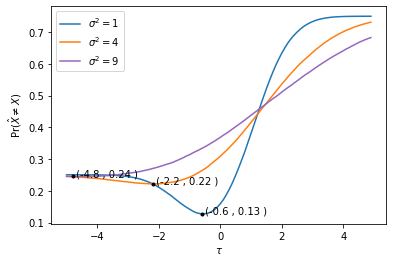
\includegraphics[width=0.4\textwidth]{fig-errorVstau}
    \caption{Plot to show Pr$ \left( \hat{X} \neq X \right)$ is minimum at negative value of $\tau$ for all nonzero values of $\sigma^2$}
    \label{fig:errorVstau}
\end{figure}
\newpage
\begin{figure}[h!]
    \centering
    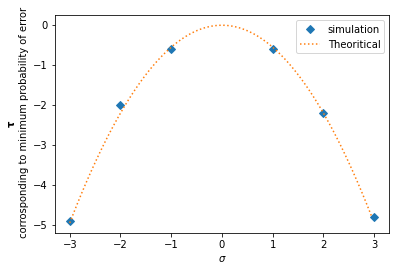
\includegraphics[width=0.4\textwidth]{fig-tauVssigma}
    \caption{Plot to show $\tau=-\frac{\sigma^2 \ln{3}}{2}$ corresponds to minimum probability of error}
    \label{fig:my_label}
\end{figure}
\end{document}